\documentclass[conference]{IEEEtran}
\IEEEoverridecommandlockouts
% The preceding line is only needed to identify funding in the first footnote. If that is unneeded, please comment it out.
\usepackage{cite}
\usepackage{amsmath,amssymb,amsfonts}
\usepackage{algpseudocode}
\usepackage{algorithm}
\usepackage{graphicx}
\usepackage{textcomp}
\usepackage{xcolor}
\usepackage{nicefrac}
\usepackage[frozencache,cachedir=.]{minted}
\usepackage{pgfplots}
\usepackage[english]{babel}
\usepackage{amsthm}
\usepackage{booktabs}

\newtheorem{theorem}{Theorem}
\newtheorem{corollary}{Corollary}[theorem]
\newtheorem{lemma}[theorem]{Lemma}

\newcommand{\floor}[1]{\lfloor #1 \rfloor}
\newcommand{\ceil}[1]{\lceil #1 \rceil}

\graphicspath{{./figures/}}

\def\BibTeX{{\rm B\kern-.05em{\sc i\kern-.025em b}\kern-.08em
    T\kern-.1667em\lower.7ex\hbox{E}\kern-.125emX}}
\begin{document}

%\title{Accelerate Off-policy Reinforcement Learning on Multicore Shared Memory System*\\
% {\footnotesize \textsuperscript{*}Note: Sub-titles are not captured in Xplore and
% should not be used}
%\thanks{This work is supported by xxx under award xxx.}
%}

\title{Parallel Actors and Learners: A Framework for Generating Scalable RL Implementations*\\
% {\footnotesize \textsuperscript{*}Note: Sub-titles are not captured in Xplore and
% should not be used}
\thanks{This work has been sponsored by the U.S. Army Research Office (ARO) under award number W911NF1910362 and the U.S. National Science Foundation (NSF) under award numbers 2009057.}
}

\author{\IEEEauthorblockN{Chi Zhang}
\IEEEauthorblockA{\textit{Department of Computer Science} \\
\textit{University of Southern California}\\
Los Angeles, USA \\
zhan527@usc.edu}
\and
\IEEEauthorblockN{Sanmukh Rao Kuppannagari, Viktor K Prasanna}
\IEEEauthorblockA{\textit{Department of Electrical and Computer Engineering} \\
\textit{University of Southern California}\\
Los Angeles, USA \\
kuppanna@usc.edu, prasanna@usc.edu}
}

\maketitle

\begin{abstract}
Reinforcement Learning (RL) has achieved significant success in application domains such as robotics, games and health care. However, training RL agents is very time consuming. Current implementations exhibit poor performance due to challenges such as irregular memory accesses and thread-level synchronization overheads on CPU.
In this work, we propose a framework for generating scalable reinforcement learning implementations on multi-core systems. Replay Buffer is a key component of RL algorithms which facilitates storage of samples obtained from environmental interactions and data sampling for the learning process. We define a new data structure for Prioritized Replay Buffer based on $K$-ary sum tree that supports asynchronous parallel insertions, sampling, and priority updates. To address the challenge of irregular memory accesses, we propose a novel data layout to store the nodes of the sum tree that reduces the number of cache misses. Additionally, we propose \textit{lazy writing} mechanism to reduce thread-level synchronization overheads of the Replay Buffer operations. Our framework employs parallel actors to concurrently collect data via environmental interactions, and parallel learners to perform stochastic gradient descent using the collected data. Our framework supports a wide range of reinforcement learning algorithms including DQN, DDPG, etc. We demonstrate the effectiveness of our framework in accelerating RL algorithms by performing experiments on CPU + GPU platform using OpenAI benchmarks. 
Our results show that the performance of our $K$-ary sum tree based Prioritized Replay Buffer improves the baseline implementations by around 4x$\sim$100x. Our proposed synchronization optimizations improve the performance by around 2x$\sim$4.4x compared with using a global lock. 
By plugging our Replay Buffer implementation into existing open source reinforcement learning frameworks, we achieve 1.19x$\sim$1.75x speedup for various algorithms.

    % Reinforcement Learning (RL) has achieved significant success application domains such as robotics, games, health care and others. 
    % However, training RL agents is very time consuming, e.g it takes weeks to train AlphaZero on hundreds of GPUs.
    % Prior works focus on parallelizing reinforcement learning on clusters while the acceleration on multicore platforms is left unexplored.
    % Replay Buffer is a key component of off-policy RL algorithms which facilitates storage of samples obtained from environmental interactions and their sampling for the learning process. 
    % However, its current implementations exhibit poor performance due to challenges such as irregular memory accesses and synchronization overheads. 
    % In this work, we propose a framework for generating scalable reinforcement learning implementations on multicore systems.
    % % Compared with clusters, data communication is significantly reduced due to the benefit of shared memory.
    % We define a new data structure for prioritized replay buffer based on K-ary sum tree that supports asynchronous parallel insertion, sampling, and priority update.
    % To address the challenge of irregular memory accesses, we propose a novel data layout to store the nodes of the sum tree that reduces the number of cache misses.
    % Additionally, we propose \textit{lazy writing} mechanism to reduce synchronization overheads of the replay buffer: only lightweight bookkeeping is performed when acquiring the lock and heavyweight workloads such as data writing are postponed after releasing the lock.
    % Our framework employs parallel actors to collect the data in the environment concurrently and parallel learners to perform stochastic gradient descent. 
    % Given hardware configurations, our framework automatically allocates the number of threads for actors and learners such that the desired ratio between the throughput of the data collection and the throughput of the learning is satisfied.
    % Our framework supports a wide range of reinforcement learning algorithms including DQN, DDPG, TD3, SAC and so on.
    % We demonstrate the effectiveness of our framework in accelerating off-policy RL algorithms by performing experiments on xxx platform using Atari benchmarks.
    % Our results shows that the performance of our approach scales in linear with the number of cores. 
    % Compared with the baseline approaches, we reduce the convergence time by $x\%\sim x\%$. 
    % By plugging our replay buffer implementation into existing open source reinforcement learning frameworks, we achieve $x\%\sim x\%$ speedup.
\end{abstract}

\begin{IEEEkeywords}
parallel reinforcement learning, prioritized replay buffer, parameter server
\end{IEEEkeywords}

\section{Introduction}
Reinforcement Learning (RL) has shown great success in a wide range of applications including board games \cite{alphago}, strategy games \cite{alphastarblog}, energy systems \cite{chi_buildsys19}, robotics \cite{rl_robots_nn}, recommendation systems \cite{recommendation_rl}, hyperparameter selection \cite{effective_online_hyperparameter} etc. Typically, RL algorithms train by iteratively collecting the data by interacting with a simulator of the environment, and learning a model using the collected data. However, it takes a considerable amount of time to train a reinforcement learning agent to converge. This is because: 1) the speed of data collection is limited by the complexity of the environment simulator which needs to accurately represent the real world physical system; 2) the large state space needed to represent a typical real-world physical system makes it necessary to gather a large amount of data to successfully train a RL agent.  We show the training time versus the size of the state space of three popular environments used in RL training in Figure~\ref{fig:time_vs_state_space}. On Mujoco~\cite{mujoco}, which is a physics engine to simulate robotics, biomechanics, etc., it takes around 3 hours to train an agent using Pytorch \cite{pytorch} on a 4-core machine with a GTX 1060 GPU. On Atari~\cite{openai_gym}, which is a game simulator, it takes around 12 hours to train on the same machine. The state-of-the-art RL algorithm for playing Go --- AlphaGo Zero~\cite{alphago_zero} was trained on 4 TPUs \cite{tpu} for 21 days. Thus, developing faster reinforcement learning algorithms is an important research direction.


%1) the speed of data collection by interacting with the environment is constrained by hardware and rules (e.g. self-driving cars can drive at most 65 MPH in freeway at Los Angeles.); 2) the large state space makes it necessary to gather large amount of data to successfully train a reinforcement learning agent. 


 
%It takes around 3 hours to train an agent to tackle Mujoco \cite{mujoco} tasks using Pytorch \cite{pytorch} on a 4-core machine with a GTX 1060 GPU. 
%It takes around 12 hours to tackle Atari games \cite{openai_gym} on the same machine. 
%The state-of-the-art AlphaGo Zero \cite{alphago_zero} was trained on 4 TPUs \cite{tpu} for 21 days. Due to the computational expensiveness, developing parallel algorithms to accelerate the reinforcement learning algorithms becomes promising and critical.

Prior work tackles this problem by deploying parallel actors that can collect data simultaneously \cite{gorila, apex, a3c, impala}. \cite{gorila} introduces a parallel framework for Deep Q Network (DQN) \cite{dqn}. 
It accelerates the training by using independent actors collecting data asynchronously. The data is stored in a shared replay buffer. 
Meanwhile, parallel learners sample data uniformly from the replay buffer and compute the gradients. 
The gradients are sent to the central parameter server \cite{parameter_server} for neural network weights update.
\cite{apex} improves the performance of \cite{gorila} by using Prioritized Replay Buffer so that important data is sampled with higher weights to accelerate the training.

In these works, Replay Buffer management becomes a limiting factor in achieving high scalability when increasing parallelism. Improving the performance of parallel Replay Buffer management via techniques such as careful data structure design or low overhead thread-level synchronization has not received much attention. In this work, we optimize the implementation of Replay Buffer management and propose a framework for generating scalable reinforcement learning implementations. The generated RL implementations are composed of parallel actors and learners executing on computing platforms such as CPUs, GPUs, or FPGAs with Replay Buffer management executing on a CPU platform. We illustrate our framework by generating RL algorithms targeting a multi-core platform. Our key contributions are summarized as follows:
\begin{itemize}
    \item We propose a new data structure for the Prioritized Replay Buffer based on $K$-ary sum tree that supports asynchronous parallel insertions, sampling and priority update.
    \item We propose a novel data layout to store the nodes of the sum tree to minimize the number of cache misses.
    \item We propose \textit{lazy writing} mechanism to minimize the thread-level synchronization overhead of various operations of the Replay Buffer.
    \item Given a hardware configuration, our framework automatically decides the number of actors and learners such that the desired ratio between the throughput of the data collection and the throughput of the learning is achieved.
    \item Our framework supports a wide range of reinforcement learning algorithms including DQN \cite{dqn}, DDQN \cite{double_q_learning}, DDPG \cite{ddpg}, TD3 \cite{td3}, SAC \cite{sac}, etc.
  %  \item Given hardware resources, we perform design space exploration to determine the number of cores to run actors and the number of cores to run learners such that the throughput of the data collection matches the throughput of the learning.
    \item We demonstrate the effectiveness of our framework in accelerating RL algorithms by performing experiments on CPU + GPU platforms using OpenAI \cite{openai_gym} benchmarks. Our results show that the performance of our $K$-ary sum tree based Prioritized Replay Buffer improves the baseline implementations by around 4x$\sim$100x. Our proposed synchronization optimizations improve the performance by around 2x$\sim$4.4x compared with using a global lock. By plugging our Replay Buffer implementation into existing open source reinforcement learning frameworks, we achieve 1.19x$\sim$1.75x speedup for various algorithms.
\end{itemize}



%This is because these works lack detailed 


%Most prior works are either specialized for a particular algorithm or lack detailed synchronization mechanisms and data structure designs that support parallelism.
%In this work, we propose a framework for generating scalable reinforcement learning implementations on multicore platforms.
%Our key contributions are summarized as follows:


\begin{figure}
    \centering
    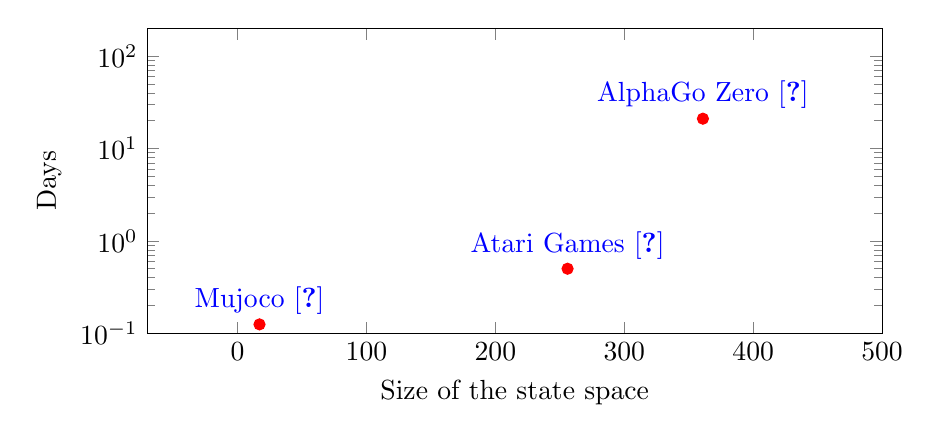
\begin{tikzpicture}
        \begin{axis}[
            ymode=log,
            xmin = -70, xmax = 500,
            ymin = 0.1, ymax = 200,
            xlabel={Size of the state space},
            ylabel={Days},
            % grid = both,
            % xmajorgrids=true,
            % major grid style = {lightgray},
            % minor grid style = {lightgray},
            width = 0.9\linewidth,
            height = 0.45\linewidth,
            nodes near coords=\pgfplotspointmeta,
            point meta=explicit symbolic
        ]
        \addplot[scatter,only marks,mark options={scale=1,fill=red,draw=red},color=blue] table [meta index=2] {
        4 0.01 CartPole
        17 0.125 Mujoco\cite{openai_gym}
        256 0.5 Atari\ Games\cite{openai_gym}
        361 21 AlphaGo\ Zero\cite{alphago_zero}
        };  
        \end{axis}
    \end{tikzpicture}
    \caption{Training time of various environments versus the size of the state space}
    \label{fig:time_vs_state_space}
\end{figure}


\section{Background Denoising Diffusion Probabilistic Models} \label{sec:background}
In this section we provide the mathematical foundation on denoising diffusion probabilistic models including recent advances. We will not cover continuous time score-based models nor latent diffusion models.

As stated in the introduction, diffusion models are generative deep learning models. In general, generative models are likelihood-based models, meaning they learn a data distribution that, ideally, maximizes the likelihood that the learned distribution matches the real data distribution. Specifically, diffusion models are latent variable models that learn to generate data, by sampling from a latent space distribution in a Markovian process, usually a Gaussian distribution due to its convenient closed form representation. This process is the reverse diffusion process the model must learn. The forward diffusion process, also a Markovian process, is applied during training to learn the reverse diffusion process.

%%%%%%%%%%%%%%%%%%%%%%%%%%%%%%%%%%%%%%%%%%%%%%%%%%%%%%%%%%%%%%%%%%
% Forward Diffusion Process
%%%%%%%%%%%%%%%%%%%%%%%%%%%%%%%%%%%%%%%%%%%%%%%%%%%%%%%%%%%%%%%%%%
\subsection{Forward Diffusion Process} \label{sec:forward_diffusion_process}
In the forward diffusion process, Gaussian noise $\mathcal{N}$ is repeatedly added to a input data sample $x_0$ for $t$ time steps with $\{t \in \mathbb{R} | 1 \le t \le T\}$ in a Markovian process, such that $p\left(x_T\right)=\mathcal{N}\left(x_T;0,\boldsymbol{I}\right)$.
A sample $x_t$ only depends on a sample $x_{t-1}$ and a fixed noise schedule $\beta_t$ and is defined by the forward diffusion kernel:
\begin{equation}
\label{eq:diffusion_kernel}
q\left(x_t|x_{t-1}\right) = \mathcal{N}\left(x_t;\sqrt{1-\beta x_{t-1}},\beta_t \boldsymbol{I}\right)
\end{equation}

The joint distribution $q\left(x_{1:T}|x_{0}\right)$ of all samples generated on the trajectory of the Markovian forward diffusion process is defined as the product of the diffusion kernel at each time step $t$:
\begin{equation}
q\left(x_{1:T}|x_{0}\right) = \prod_{t=1}^{T} q\left(x_t|x_{t-1}\right)
\end{equation}

Equation \eqref{eq:diffusion_kernel} can be simplified to be able to generate a noisy sample at any given time step $t$ only conditioned on $x_0$:
\begin{equation}
\label{eq:diffusion_kernel_simplified}
\begin{aligned}
q\left(x_{t}|x_{0}\right) &= \mathcal{N}\left(x_t;\sqrt{\bar{\alpha}_t}x_0,\left(1-\bar{\alpha}_t \right) \boldsymbol{I}\right) \\
\bar{\alpha}_t &= \prod_{s=1}^{t} \left(1-\beta_t\right)
\end{aligned}
\end{equation}

The noise schedule $\beta_{t}$ is selected in such a way, that for $T$ time steps, $\bar{\alpha_T}$ approaches 0, which, according to \eqref{eq:diffusion_kernel_simplified}, results in a standard normal distribution $\mathcal{N}\left(0,\boldsymbol{I}\right)$ for $q\left(x_{T}|x_{0}\right)$. The shape of the noise schedule is a hyperparameter to be selected. While \cite{ho_denoising_2020} uses a linear schedule, \cite{nichol_improved_2021} proposes a cosine schedule.

To be able to calculate gradients of a stochastic variable in the back-propagation step during training, it is required to apply the reparameterization trick for sampling from a Gaussian distribution. A sample $x_t$ at a given time step $t$ can be formulated as:
\begin{equation}
x_{t} = \sqrt{\bar{\alpha}_t}x_0 + \sqrt{\left(1-\bar{\alpha}_t\right)}\epsilon, \;  where \: \epsilon \sim \mathcal{N}\left(0,\boldsymbol{I}\right)
\end{equation}

The data distribution $q\left(x_{t}\right)$ at any time step $t$ is the joint probability of all distributions of previous time steps. Using ancestral sampling it can be reformulated to:
\begin{equation}
q\left(x_{t}\right) = \int q\left(x_{0},x_{t}\right) dx_0 = \int q\left(x_{0}\right) q\left(x_{t}|x_{0}\right) dx_0
\end{equation}
In other words, to draw a sample $x_t \sim q\left(x_{t}\right)$, one can first draw $x_0 \sim q\left(x_{0}\right)$, which is basically drawing a sample from the input dataset, and then draw a sample $x_t$ from $q\left(x_{t}|x_0\right)$, which is the forward diffusion from equation \eqref{eq:diffusion_kernel_simplified}. 


%%%%%%%%%%%%%%%%%%%%%%%%%%%%%%%%%%%%%%%%%%%%%%%%%%%%%%%%%%%%%%%%%%
% Reverse Diffusion Process
%%%%%%%%%%%%%%%%%%%%%%%%%%%%%%%%%%%%%%%%%%%%%%%%%%%%%%%%%%%%%%%%%%
\subsection{Reverse Diffusion Process} \label{sec:reverse_diffusion_process}

For DDPMs, the reverse diffusion process is Markovian, similar to that of the forward diffusion process. 
The naive approach is to draw the initial sample $x_T \sim \mathcal{N}\left(x_T;\boldsymbol{0},\boldsymbol{I}\right)$ and then iteratively draw a less noisy sample $x_{t-1} \sim q\left(x_{t-1}|x_{t}\right)$. The issue is that $q\left(x_{t-1}|x_{t}\right)$ is intractable, meaning there is no closed form solution. Diffusion models solve this issue by learning the intractable posterior distribution parameterized by $\theta$ given as:
\begin{equation}
\label{eq:intractable_posterior_distribution}
p_{\theta}\left(x_{t-1}|x_t\right) = \mathcal{N}\left(x_{t-1};\mu_{\theta}\left(x_t,t\right),\Sigma_{\theta}\left(x_t,t\right)\right)
\end{equation}

and its corresponding joint distribution
\begin{equation}
\label{eq:joint_reverse_distribution}
p_{\theta}\left(x_{1:T}|x_{0}\right) = p\left(x_{T}\right)\prod_{t=1}^{T} p_{\theta}\left(x_{t-1}|x_{t}\right)
\end{equation}

The diffusion model is trained by optimizing the variational bound of the negative log-likelihood: 
\begin{equation}
\begin{aligned}
L & := \mathbb{E}_{q\left(x_{0}\right)}\left[-log\, p_{\theta}\left(x_{0}\right)\right] \\
  & \le \mathbb{E}_{q\left(x_{0}\right)q\left(x_{1:T}|x_0\right)}\left[-log\frac{p_{\theta}\left(x_{0:T}\right)}{q\left(x_{1:T}|x_0\right)}\right]
\end{aligned}
\end{equation}

which can be rewritten as
\begin{equation}
\label{eq:variational_lower_bound}
\begin{aligned}
L_{VLB} & := \mathbb{E}_{q}\left[L_{0} + L_{t-1} + L_{T}\right] \\
L_{0} & := -log\, p_{\theta}\left(x_{0}|x_{1}\right)\\
L_{t-1} & := \sum_{t<1}D_{KL}\left(q\left(x_{t-1}|x_t,x_0\right)\|p_{\theta}\left(x_{t-1}|x_t\right)\right)\\
L_{T} & := D_{KL}\left(q\left(x_{T}|x_0\right)\|p\left(x_{T}\right)\right)
\end{aligned}
\end{equation}
where $D_{KL}\left(\|\right)$ is the Kullback-Leibler(KL)-Divergence between two distributions and $q\left(x_{t-1}|x_t,x_0\right)$ is the tractable posterior distribution
\begin{equation}
q\left(x_{t-1}|x_t,x_0\right) = \mathcal{N}\left(x_{t-1};\Tilde{\mu}_t\left(x_t,x_0\right),\Tilde{\beta}_t\boldsymbol{I}\right)
\end{equation}
where
\begin{equation}
\begin{aligned}
\Tilde{\mu}_t\left(x_t,x_0\right) & := \frac{\sqrt{\bar{\alpha}_{t-1}}\beta_t}{1-\bar{\alpha}_{t}}x_0 + \frac{\sqrt{1-\beta_t}\left(1-\bar{\alpha}_{t-1}\right)}{1-\bar{\alpha}_{t}}x_t \\
\Tilde{\beta}_t & := \frac{1-\bar{\alpha}_{t-1}}{1-\bar{\alpha}_{t}}\beta_t
\end{aligned}
\end{equation}

In other words, $\Tilde{\mu}_t\left(x_t,x_0\right)$ is the weighted sum of an unnoisy sample $x_0$ and a noisy sample $x_t$ at time step $t$.

Equation \eqref{eq:variational_lower_bound} can be further simplified by setting $L_T=0$, since the Kullback-Leibler-Divergence of two Gaussians is zero under the assumption that $q\left(x_{T}|x_0\right) \approx \mathcal{N}\left(\boldsymbol{0},\boldsymbol{I}\right)$ and $p\left(x_{T}\right) \approx \mathcal{N}\left(\boldsymbol{0},\boldsymbol{I}\right)$, which previously has been defined to be the case.

The better the model learns to approximate the parameterized denoising posterior distribution $p_{\theta}\left(x_{t-1}|x_t\right)$ with the real tractable denoising posterior distribution $q\left(x_{t-1}|x_t,x_0\right)$, the smaller the KL-divergence and hence the smaller $L_{VLB}$.
Since all distributions in \eqref{eq:variational_lower_bound} are tractable and all KL-Divergences are comparisons of Gaussians, they can be calculated in closed form:
\begin{equation}
\label{eq:closed_form_lt-1}
\begin{aligned}
L_{t-1} & = D_{KL}\left(q\left(x_{T}|x_0\right)\|p\left(x_{T}\right)\right) \\
        & = \mathbb{E}_{q}\left[\frac{1}{2\sigma^2_t}\|\Tilde{\mu}_t\left(x_t,x_0\right)-\Tilde{\mu}_{\theta}\left(x_t,t\right)\|^2\right] + const
\end{aligned}
\end{equation}

\cite{ho_denoising_2020} found that predicting the noise $\epsilon$ that was applied in the forward diffusion to reverse the diffusion process by using a noise predictor $\epsilon_{\theta}$ works best and modified \eqref{eq:closed_form_lt-1} to:
\begin{equation}
\begin{aligned}
L_{t-1} = \mathbb{E}_{q}\left[\lambda_t\frac{\beta_t}{\left(1-\beta_t\right)\left(1-\alpha_t\right)}\|\epsilon-\epsilon_{\theta}\left(x_t,t\right)\|^2\right] + const
\end{aligned}
\end{equation}

\cite{ho_denoising_2020} further observed that setting the time dependent scalar $\lambda_t=\left(1-\beta_t\right)\left(1-\alpha_t\right)/\beta_t$, improves sample quality and simplifies the training objective to:
\begin{equation}
\label{eq:loss_simple}
\begin{aligned}
L_{simple} = \mathbb{E}_{q}\left[\|\epsilon-\epsilon_{\theta}\left(x_t,t\right)\|^2\right].
\end{aligned}
\end{equation}

In contrast to \cite{ho_denoising_2020}, \cite{choi_perception_2022} proposes a more sophisticated choice of $\lambda_t$, namely P2 weighting, to prioritizes different noise levels to improve the sample quality:
\begin{equation}
\lambda'_t = \frac{\lambda_t}{\left(k+SNR(t)\right)^{\gamma}}
\end{equation}
where $k$ is a hyper parameter to prevent exploding weights, $\gamma$ controls the strength of down weighting and the signal-to-noise ratio $SNR(t)=\alpha_t/(1-\alpha_t)$ is a simplified expression for the noise schedule by \cite{kingma_variational_2022}.

While \cite{ho_denoising_2020} only predicts the mean of the added noise and sets the variance to be either $\beta_t$ or $\Tilde{\beta}_t$ the upper and lower variational bound respectively, \cite{nichol_improved_2021} found that learning the variance $\Sigma_{\theta}\left(x_t,t\right)$ from equation \eqref{eq:intractable_posterior_distribution} improves sample quality and allows sampling with a reduced number of time steps with little change in sample quality. Instead of predicting $\Sigma_{\theta}\left(x_t,t\right)$ directly, they propose to learn the variance as a weighted sum of the upper and lower bound using a neuronal network's output $v$:
\begin{equation}
\Sigma_{\theta}\left(x_t,t\right) = exp\left(v\,log\,\beta_t+\left(1-v\right)log\,\beta_t\right)
\end{equation}

Since $L_{simple}$ does not provide a learning signal for $\Sigma_{\theta}\left(x_t,t\right)$, \cite{nichol_improved_2021} proposes a hybrid loss function:
\begin{equation}
L_{hybrid} = L_{simple} + \lambda L_{VLB}
\end{equation}

To sample a less noisy sample $x_{t-1}\sim p_{\theta}\left(x_{t-1}|x_t\right)$ the trained diffusion model $\epsilon_{\theta}$ estimates the noise that was added from time step $t-1$ to $t$ and subtracts that noise from $x_t$.
\begin{equation}
x_{t-1} = \frac{1}{\sqrt{\alpha_t}}\left(x_t - \frac{1-\alpha_t}{\sqrt{1-\bar{\alpha}_t}}\epsilon_{\theta}(x_t,t)\right) + \sigma_t z
\end{equation}
%where $ z \sim \mathcal{N}\left(\boldsymbol{0},\boldsymbol{I}\right) $
where $ z \sim \mathcal{N}\left(\boldsymbol{0},\boldsymbol{I}\right) $

%%%%%%%%%%%%%%%%%%%%%%%%%%%%%%%%%%%%%%%%%%%%%%%%%%%%%%%%%%%%%%%%%%
% Conditional Diffusion Process
%%%%%%%%%%%%%%%%%%%%%%%%%%%%%%%%%%%%%%%%%%%%%%%%%%%%%%%%%%%%%%%%%%
\subsection{Conditional Diffusion Process} \label{sec:conditional_diffusion_process}
All previous formulations describe the unconditional case, where unconditional means no extra condition beside the Markovian process. The ultimate goal of a generative model is to control the sampling process by incorporating a condition $c$ to obtain a desired output.

The reverse process from equations \eqref{eq:intractable_posterior_distribution} and \eqref{eq:joint_reverse_distribution} can be extended as follows:
\begin{equation}
\begin{aligned}
p_{\theta}\left(x_{t-1}|x_t, c\right) & = \mathcal{N}\left(x_{t-1};\mu_{\theta}\left(x_t,t,c\right),\Sigma_{\theta}\left(x_t,t,c\right)\right) \\
p_{\theta}\left(x_{0:T}|c\right) & = p\left(x_{T}\right)\prod_{t=1}^{T} p_{\theta}\left(x_{t-1}|x_{t},c\right)
\end{aligned}
\end{equation}

Similarly, the variational lower bound from equation \eqref{eq:variational_lower_bound} is extends to:
\begin{equation}
\label{eq:variational_lower_bound_conditional}
\begin{aligned}
L_{VLB} & := \mathbb{E}_{q}\left[L_{0} + L_{t-1} + L_{T}\right] \\
L_{0} & := -log\, p_{\theta}\left(x_{0}|x_{1},c\right)\\
L_{t-1} & := \sum_{t<1}D_{KL}\left(q\left(x_{t-1}|x_t,x_0\right)\|p_{\theta}\left(x_{t-1}|x_t,c\right)\right)\\
L_{T} & := D_{KL}\left(q\left(x_{T}|x_0,c\right)\|p\left(x_{T}\right)\right)
\end{aligned}
\end{equation}

\section{Related Work} \label{sec:related_work}
%In this section we put our work into a broader context and provide a summary of other related work, which by no means we claim to be extensive, but rather an overview.
In this section, we situate our work within a broader context and offer a concise summary of other relevant studies.

% DDPMs 
\subsection{Denoising Diffusion Probabilistic Models} Denoising diffusion models are a type of generative deep learning models first formulated by \cite{sohl-dickstein_deep_2015} and further extended to Denoising Diffusion Probabilistic models (DDPMs) by \cite{ho_denoising_2020,nichol_improved_2021}. These models use a Markov Chain to gradually convert one simple and well-known distribution (e.g. a Gaussian distribution) into a usually more complex data distribution the model can sample from. 

% diffusion applications
Diffusion models have been applied to many applications and modalities including image generation \citep{dhariwal_diffusion_2021}, image-to-image translation \citep{saharia_palette_2022}, super-resolution \citep{ho_cascaded_2021, saharia_image_2021}, video \citep{ho_video_2022,harvey_flexible_2022,yang_diffusion_2022}, audio \citep{kong_diffwave_2021,lee_priorgrad_2022}, text-to-image \citep{ramesh_hierarchical_2022, nichol_towards_2022,saharia_photorealistic_2022}, and simultaneous multi-modal generation \citep{ruan_mm-diffusion_2023}.

% generative trilemma
In the generative learning trilemma formulated by \cite{xiao_tackling_2022}, which states that generative models cannot satisfy all three key requirements fast sampling, high quality samples and mode coverage, diffusion models have shown good results in high quality image generation \citep{rampas_novel_2023,ho_cascaded_2021} and mode coverage. While Variational Auto-Encoders (VAEs) \citep{kingma_auto-encoding_2022,razavi_generating_2019} and flow based models \citep{dinh_density_2017,durkan_neural_2019} are strong in covering multi-modal data distributions and can be sampled from very fast, the quality of their samples is usually not as high as of Generative Adversarial Models (GANs) or diffusion models. GANs \citep{goodfellow_generative_2014,brock_large_2019,kirch_vologan_2022} on the other-hand produce high quality images and are sampled quickly but are prone to mode collapse and often do not cover the entire data distribution.

% speed up sampling
DDPMs require many reverse diffusion steps (often several hundreds or even thousands of steps) to sample from, making it difficult train and deploy them even on modern GPUs. Hence it is no surprise that a lot of research focuses on increasing the sample speed of diffusion models by reducing the number of required steps \citep{song_denoising_2022, xiao_tackling_2022, nichol_improved_2021, salimans_progressive_2022,chung_come-closer-diffuse-faster_2022}, perform diffusion in the latent space rather than the full-resolution data distribution \citep{preechakul_diffusion_2022,rombach_high-resolution_2022,sinha_d2c_2021, gu_vector_2022, tang_improved_2023} or formulate the diffusion problem as time-continuous problem to take advantage of accelerated stochastic differential equations (SDE) solvers \citep{song_score-based_2021,song_maximum_2021, song_improved_2020,karras_elucidating_2022}.

% conditional generation
To control the output of the model it must be provided with an additional condition input. The model might be conditioned on another input of the same modality like in colorization \citep{saharia_palette_2022}, inpaintings \citep{batzolis_conditional_2021}, generation from semantic mask \citep{meng_sdedit_2022} or image super-resolution \citep{saharia_image_2021,ho_cascaded_2021}, on an input of different modality like in depth estimation \citep{duan_diffusiondepth_2023} or segmentation \citep{baranchuk_label-efficient_2022}, on class labels \citep{dhariwal_diffusion_2021} or on text prompts \citep{ramesh_hierarchical_2022, nichol_towards_2022,saharia_photorealistic_2022}; to name a few.

Depending on the representation of the condition input, it might be concatenated with the noise input \citep{batzolis_conditional_2021}, fed to multiple layers within the network like adaptive instance normalization \citep{karras_style-based_2019} or via an independent network branch \citep{zhang_adding_2023}. Beside the architectural choice one must also decide how strong the condition should be. One could only apply it for certain time steps in the reverse diffusion process, only apply it during inference on an unconditionally trained model \citep{choi_ilvr_2021} or using guidance, which applies a weighted sum of a conditional and unconditional generation and hence trades-off sample diversity with sample quality. Among others, guidance can be performed with an additionally trained classifier \citep{nichol_improved_2021}, by training the diffusion model conditionally and unconditionally at the same time and sampling using a weighted sum of both \citep{ho_classifier-free_2022} or by using pre-trained CLIP embeddings \citep{nichol_towards_2022,ramesh_hierarchical_2022}.

% Monocular depth estimation
\subsection{Monocular Depth Estimation} Knowledge on the depth of a scene is crucial in a vast number of applications including virtual reality (VR), augmented reality (AR), environment perception, autonomous driving, robotics, state estimation, navigation, mapping and many more. Various surveys \citep{bhoi_monocular_2019,zhao_monocular_2020,ming_deep_2021, masoumian_monocular_2022} summarize the rich and extensive literature on monocular depth estimation; the estimation of the depth based on a single image; an inherently ill-posed and ambiguous problem.

In contrast, conventional geometric-based approaches such as structure from motion and stereo vision matching rely on geometric constraints and multiple viewpoints to reconstruct 3D structures. On the other hand, sensor-based methods leverage dedicated hardware like LiDAR sensors or RGB-D cameras to directly capture depth information. While these methods find practical application, they suffer from significant limitations including high hardware expenses, imprecise and sparse predictions, and limited accessibility for consumer use.

Many different representations can be deployed to obtain depth information: 2D depth maps (dense or sparse), 3D point cloud, 3D pseudo point cloud predicted from other modality (e.g. stereo camera), camera independent disparity maps, light fields, neural radiance fields (NERFs, \cite{mildenhall2021nerf}), 3D meshes, voxels and height maps to name a few.

Numerous deep learning based approaches for monocular depth estimation have been researched in recent years. 
\cite{lu_self-supervised_2022}, \cite{chen_self-supervised_2018} and \cite{zhang_unsupervised_2020} train their models using stereo images while inferring only single view images. The model either learns the correspondence between the two views and can reconstruct the other view or the model incorporates the knowledge of a stereo camera into its weights and hence strengthen its capability to extract meaningful features from a single image. \cite{yue_self-supervised_2022} and \cite{ zhao_joint_2022} apply a multi-task training objective by not only predicting depth but also other related tasks (e.g. normal vector prediction) that help the model to learn a more profound representation and understanding of the scene which also benefits the downstream task of depth estimation.
\cite{watson_temporal_2021} and \cite{bian_unsupervised_2021} use mono camera videos to estimate the depth.

Other deep learning-based approaches focus on multiple sensor modalities to estimate the depth of the scene. \cite{zhang_lidar-guided_2022} use LiDAR point clouds in combination with stereo images, \cite{eldesokey_confidence_2020} use monocular RGB images combined with sparse LiDAR point clouds, \cite{liu_pseudo-lidar_2020} input monocular RGB combined with a depth map and \cite{piao_dynamic_2021} combine a single RGB image with a focal stack.

In this work, we focus on monocular depth estimation using single RGB images as input and generating dense depth maps as output.
We observed that most model architectures are based on GANs, VAEs or similar approaches. We hence further review the usage of diffusion models in the field of depth estimation.

% Depth Diffusion
\subsection{Depth Diffusion}
We observe that very little work has been published on monocular depth estimation using diffusion models. We hypothesize that one of the major reasons is the necessity for fast sampling constraint by real-time applications like autonomous driving. We are certain that the community will find a way to further increase the sampling speed in a future and hence we see great potential in diffusion models for monocular depth estimation.

\cite{saxena_monocular_2023} used a diffusion model to perform monocular depth estimation on indoor and outdoor scenes introducing a preprocessing step to complete incomplete depth data and were even able to resolve depth ambiguity introduced from transparent surfaces.
\cite{duan_diffusiondepth_2023} use a latent diffusion model in combination with a Swin Transformer backbone \citep{liu_swin_2021} to first encode the depth into latent space and then perform the reverse diffusion in the latent space by iteratively applying their light weighted monocular conditioned denoising block. Finally, they apply a fully convolutional decoder on the diffused latent space to obtain the final depth prediction.
\cite{ranftl_towards_2020} propose methods to mix multiple depth datasets for robust training to mitigate the challenges of acquiring dense ground truth data from a variety of scenes. \cite{bhat_zoedepth_2023} proposes a method to combine relative depth and metric depth in a zero-shot manner, by pre-training on a large corpus of relative depth datasets and finetuning on metric depth.

Not as closely related but still applying diffusion models on 3D related data representations, we found \textbf{3D point cloud generation} conditioned on monocular images \citep{zhou_3d_2021}, conditioned on an encoded shape latent \citep{luo_diffusion_2021} and conditioned in CLIP-tokens \citep{nichol_point-e_2022}, \textbf{novel view synthesis} from a single view \citep{rockwell_pixelsynth_2021,watson_novel_2022}, for perpetual view generations for long camera trajectories where depth is predicted as an intermediate representation \citep{liu_infinite_2021} or combining text prompts for 2D generation with Neural Radiance Fields (NeRFs) \citep{poole_dreamfusion_2022}, \textbf{depth estimation} from multiple camera images at different viewpoints \citep{khan_differentiable_2021} and \textbf{depth-aware guidance} methods that guide the image generation process by its intermediate depth representation \citep{kim_dag_2023}.

\begin{algorithm}[!t]
    \caption{Key operations of the N-ary sum tree.}
    \label{alg:n_nary_sum_tree_func}
    \begin{algorithmic}[1]
      \Function{updateValue}{idx, value}
          \State node\_idx = \Call{convertToNodeIdx}{idx};
          \State $\Delta$ = value - \Call{getValue}{node\_idx};
          \While{!\Call{isRoot}{node\_idx}}
              \State new\_value = \Call{getValue}{node\_idx} + $\Delta$;
              \State \Call{SetValue}{node\_idx, new\_value};
              \State node\_idx = \Call{getParent}{node\_idx};
          \EndWhile
      \EndFunction
      \\
      \Function{getPrefixSumIdx}{prefixSum}
          \State node\_idx = \Call{getRoot}{\null};
          \While{!isLeaf(node\_idx)}
              \State node\_idx = \Call{getLeftChild}{node\_idx};
              \State partialSum = 0;
              \For{$i$ = 0; $i$ $<$ fan\_out; $i++$}
                  \State sum = partialSum + \Call{getValue}{node\_idx};
                  \If{sum $\geq$ prefixSum}
                      \State break;
                  \EndIf
                  \State partialSum = sum;
                  \State node\_idx = \Call{getNextSibling}{node\_idx};
              \EndFor
              \State prefixSum = prefixSum - partialSum;
          \EndWhile
          \State idx = \Call{convertToDataIdx}{node\_idx};
          \State \Return idx;
      \EndFunction
    \end{algorithmic}
\end{algorithm}

\section{Parallel Prioritized Replay Buffer}\label{sec:parallel_per}
In this section, we discuss in detail the design of our Prioritized Replay Buffer that supports parallel actors and learners. We start by introducing the key operations that need to be supported.
\subsection{Operations}\label{sec:parallel_per_ops}
\subsubsection{Insertion}
Given a new data item $x$, find the next available index $i$ and insert $x$ at $i$. If the Replay Buffer is full, find the index using the eviction policy. Set the priority at index $i$ to $P(i)=P_{\max}$, where $P(i)$ is the priority at index $i$ and $P_{\max}$ is the maximum priority in the Replay Buffer. The most common eviction policy used in existing implementations is First-in-first-out (FIFO).
\subsubsection{Sampling}
Sample a data item $x_i$ according to the probability distribution $Pr(i)=\nicefrac{P(i)}{\sum_{i}P(i)}, i=1,2,\ldots, N$, where $N$ is the size of the Replay Buffer. To do so, we first sample $x$ from uniform distribution $U(0,1)$. Then, we compute the cumulative density function (cdf) as $cdf(i)=\sum_{j=1}^{i}Pr(j), i=1,2,\ldots, N$. Finally, the sampled index $i=cdf^{-1}(x)$. Mathematically, this is equivalent to finding the minimum index $i$, such that the \textbf{prefix sum} of the probability from 0 to $i$ is greater than or equal to $x$:
\begin{align}
    \min_{i}\sum_{j=1}^{i}Pr(i)\geq x \Rightarrow \min_{i}\sum_{j=1}^{i}P(i)\geq x\cdot \sum_{j=1}^{N}P(j)
    \label{eq:prefix_sum}
\end{align}
\subsubsection{Priority retrieval}
Return the priority at index $i$.
\subsubsection{Priority update}
Update the priority at index $i$.

\subsection{Frequency of the Operations and Runtime Requirements} 
As shown in Algorithm~\ref{alg:off_policy_rl}, the insertion is executed once per iteration. The sampling, priority retrieval and priority update are executed once every update\_interval. Directly storing the priority in an array incurs a runtime complexity of $\Theta(N)$ for sampling and $\Theta(1)$ for priority retrieval and priority update. Directly storing the prefix sum in an array incurs a runtime of $\Theta(\log N)$ in sampling, $\Theta(1)$ in priority retrieval and $\Theta(N)$ in priority update. Based on the frequency of the operations, both these implementations incur a overall runtime complexity of $\Theta(N)$. In this paper, we proposed to use $K$-ary sum tree to implement the Prioritized Replay Buffer to achieve $\Theta(\log N)$ runtime complexity for both sampling and priority update and thus for the entire implementation.

\subsection{$K$-ary Sum Tree}\label{sec:sum_tree}
We show an example of a $K$-ary sum tree for $K=4$ in Figure~\ref{fig:sum_tree}. Each node has $K$ child nodes. The value stored in the parent node is the sum of all the values stored in the child nodes. The leaf nodes hold the actual priorities. 

\begin{figure}
    \centering
    \includegraphics[width=\linewidth]{sum_tree.pdf}
    \caption{The overall structure of a 4-ary sum tree.}
    \label{fig:sum_tree}
\end{figure}

\begin{figure}
    \centering
    \includegraphics[width=\linewidth]{update_value.pdf}
    \caption{Illustration of the process when updating the value in the $K$-ary sum tree with fanout=4 as shown in Algorithm~\ref{alg:n_nary_sum_tree_func}. The blue node denotes the leaf node that holds the priority. The green nodes denote the intermediate sums that are updated by propagating the change of the priority from the leaf to the root. The red dotted arrow shows the direction of the value propagation.}
    \label{fig:update_value}
\end{figure}

\begin{figure*}
    \centering
    \includegraphics[width=\linewidth]{get_prefix_sum.pdf}
    \caption{Illustration of the process when sampling index according to the priority in the $K$-ary sum tree with fanout=4 as shown in Algorithm~\ref{alg:n_nary_sum_tree_func}. Starting from the root node, the green nodes denote the cutoff node during traversal and the blue node denotes the leaf node sampled. The red dotted arrow shows the direction of the tree traversal.}
    \label{fig:get_prefix_sum}
\end{figure*}

\subsubsection{Priority retrieval}
In order to obtain the priority for the index $i$, we create an array of pointers, each pointing to its corresponding leaf node that holds the priority value. Thus, priority retrieval using $K$-ary sum tree requires $\Theta(1)$ time.

\subsubsection{Priority update}
To update the priority of index $i$, we first obtain the leaf node holding the priority. We compute the change of the priority by subtracting the old value from the new value. Then, we propagate the change of the priority from the leaf node to the root node by traversing along the parent nodes. We show a detailed function in Algorithm~\ref{alg:n_nary_sum_tree_func} and an example in Figure~\ref{fig:update_value}. It is easy to see that this operation requires $\Theta(\log_K N)$ time.

\subsubsection{Prefix sum index computation}
Given a randomly sampled number $x\sim U(0,1)$, the objective is to compute index $i=\min_{i}\sum_{j=1}^{i}P(i)\geq x\cdot \sum_{j=1}^{N}P(j)$ as discussed in Section~\ref{sec:parallel_per_ops}. The sum of all the priorities in the Replay Buffer $\sum_{j=1}^{N}P(j)$ can be computed in $\Theta(1)$ by simply retrieving the value stored in the root node. To design an algorithm that obtains the target index, we start by proving Lemma~\ref{lemma:index_existence} and theorem~\ref{the:sum_tree_prefix}:

\begin{lemma}
    \label{lemma:index_existence}
    Let the value of the $i$-$th$ node at level $m$ be $P_{i,m}$. Assume the height of the tree is $H$. Then, at level $1\leq m\leq H$, there exists index $j$, $1 \leq j \leq K^{m-1}$, such that $\sum_{i=1}^{j}P_{m, i}\geq x\cdot \sum_{i=1}^{N}P(i)$, for any $x\in (0, 1)$.
\end{lemma}
\begin{proof}
    According to the definition, the leaf node holds the priority value. Thus, $P_{i, H}=P(i), \forall i=1,2,\ldots, K^{H-1}$. Since $x\in (0, 1)$, we obtain $x\cdot \sum_{i=1}^{N}P(i)\leq \sum_{i=1}^{N}P(i) \leq \sum_{i=1}^{K^{H-1}}P_{i,H}$. Because the priority values are non-negative, there must exist index $j$, $1 \leq j \leq K^{H-1}$, such that $\sum_{i=1}^{j}P_{H, i}\geq x\cdot \sum_{i=1}^{N}P(i)$. According to the property of the sum tree, the value of the parent is the sum of all its children. Thus, $\sum_{i=1}^{K^{H-1}}P_{H, i}=\sum_{i=1}^{K^{m-1}}P_{m, i}, \forall m=1, 2, \cdots, H-1$. Therefore, the same argument holds for each level. This concludes the proof for Lemma~\ref{lemma:index_existence}.
\end{proof}
\begin{theorem}
    \label{the:sum_tree_prefix}
    Let $j_m=\min_{j'} \sum_{i=1}^{j'}P_{m, i}\geq x\cdot \sum_{i=1}^{N}P(i)$. Then, $j_m$ is the parent node of $j_{m+1}$, $\forall m=1,2,\cdots H-1$.
\end{theorem}
\begin{proof}
    The child nodes of index $j$ at level $m$ are $K\cdot(j-1)+1,\cdots, K\cdot j$ at level $m+1$. According to the definition of the sum tree and the property of $j_m$, we obtain $\sum_{i=1}^{j_m-1}P_{m,i}=\sum_{i=1}^{K\cdot(j_m-1)}P_{m+1, i}< x\cdot \sum_{i=1}^{N}P(i)$. Thus, the index of the cutoff node at level $m+1$ must be $j_{m+1}\geq K\cdot(j_m-1)+1$. Noticing that $\sum_{i=1}^{j_m}P_{m,i}=\sum_{i=1}^{K\cdot(j_m)}P_{m+1, i}\geq x\cdot \sum_{i=1}^{N}P(i)$. Thus, the index of the cutoff node at level $m+1$ satisfies $j_{m+1}\leq K\cdot j_m$. Combining $K\cdot(j_m-1)\leq j_{m+1}\leq K\cdot j_m$, we obtain $j_m$ is the parent node of $j_{m+1}$.
\end{proof}
We refer such node $j_m$ as the \textit{cutoff node} at level $m$. The goal of sampling is to find the index of the cutoff node at the last level of the tree. 
According to Theorem~\ref{the:sum_tree_prefix}, the cutoff node at level $m$ is the parent of the cutoff node at level $m+1$. 
Therefore, we can start from the root node and perform the search only using the child nodes. To obtain which child node is the cutoff node, we maintain a cumulative sum of all the nodes left to the cutoff at each level. Please refer to Algorithm~\ref{alg:n_nary_sum_tree_func} for details.
We also illustrate an example of the process in Figure~\ref{fig:get_prefix_sum}, where $K=4$ and $H=6$.

\subsubsection{Data layout}
Maintaining the explicit tree data structure using pointers significantly degrades the cache performance of modern CPUs. In this work, we implement the tree data structure implicitly using an array as shown in Figure~\ref{fig:data_layout}. The sampling process requires traversing all the nodes under the same parent. To maximize the cache performance, it is desired that each group of child nodes under the same parent is cache aligned. Assume that one cacheline can store $C$ nodes, then we choose $K$, such that $K\%C=0$. We pad the root node with $K-1$ so that it is also cache aligned.

\begin{figure}
    \centering
    \includegraphics[width=\linewidth]{data_layout.pdf}
    \caption{Data layout of the proposed sum tree with $K=4$. The black arrow shows the first child of the parent node. The color indicates the level of the node in the tree.}
    \label{fig:data_layout}
\end{figure}

\subsubsection{Theoretical performance analysis}
\paragraph{Space complexity}
The space complexity is proportional to the number of nodes in the tree. Assume the size of the Replay Buffer is $N$, which is equal to the number of nodes in the last level of the tree. Thus, the total number of nodes in the tree is: $\Theta(\frac{K^H-1}{K-1})=\Theta(\frac{K^{H-1}\cdot K-1}{K-1})=\Theta(\frac{N\cdot K-1}{K-1})=\Theta(N+\frac{N-1}{K-1})$. Clearly, as $K$ increases, the space complexity reduces due to the decrease of the number of intermediate nodes.

\paragraph{Runtime complexity}
It is clear that the priority retrieval runs in $\Theta(1)$ and priority update runs in $\Theta(\log_K N)$. For prefix sum index computation, the loops runs $H=\ceil{\log_K N} + 1$ times. The memory access inside loop has $\nicefrac{K}{C}$ cache misses and $K\cdot(1-\nicefrac{1}{C})$ cache hit, where $C$ is the number of nodes in one cacheline. Thus, the time complexity of prefix sum index computation is $\Theta((\log_K N+1)(T_{miss}\cdot\frac{K}{C}+T_{hit}\cdot K\cdot(1-\nicefrac{1}{C})))$, where $T_{miss}$ is the execution time of one cache miss and $T_{hit}$ is the execution time of one cache hit. Note that this function has a local minimum in terms of $K$. In practice, we profile the performance of various $K$ values based on the size of the cacheline and choose the one that yields the best performance.

\subsection{Thread-safe Prioritized Replay Buffer}\label{sec:thread_safe_prb}
In order to support parallel actors and learners, it is crucial to design thread-safe prioritized Replay Buffer. We summarize the resource utilization of various operations in Table~\ref{table:resource_util}. We design the thread-safe prioritized replay buffer using locking mechanism such that the duration of holding a lock is minimized. 

\subsubsection{Synchronization of the sum tree}
We use two locks to synchronize the sum tree: one to synchronize the read/write of the last level of the tree and the other to synchronize the read/write of all the levels. A detailed procedure of priority update and priority retrieval is shown in Algorithm~\ref{alg:sync_replay_buffer}. Using this technique, reading of the priority value and updating of the intermediate levels of the sum tree can be executed in parallel. Note that it will cause inconsistencies if we acquire the global\_tree\_lock after releasing the last\_level\_lock lock when two priority update queries arrive at the same time.

\subsubsection{Synchronization of insertion and sampling}
During insertion, the Replay Buffer finds an available index. Then, it writes the data to the storage and updates the priority to the maximum priority in the Replay Buffer. Compared with index searching and priority update, data writing takes more time due to explicit copy of the memory data. Thus, it is important not to hold the lock while performing the data writing. To do so, we propose \textit{lazy writing}: 1) We set the priority to zero atomically; ii) we perform data writing; iii) we reset the priority to the maximum priority in the Replay Buffer atomically. Since the priority is zero during data writing, it will never be sampled. This makes sampling only needs to synchronize prefix sum index computation. A detailed procedure is shown in Algorithm~\ref{alg:sync_replay_buffer}.


\begin{algorithm}[!t]
    \caption{Synchronization of the Prioritized Replay Buffer}
    \label{alg:sync_replay_buffer}
    \begin{algorithmic}[1]
        \Function{PriorityUpdate}{idx, new\_priority}
            \State \Call{Acquire}{global\_tree\_lock};
            \State \Call{Acquire}{last\_level\_lock};
            \State \Call{UpdateLastLevel}{\null};
            \State \Call{Release}{last\_level\_lock};
            \State \Call{UpdateIntermediateLevel}{\null};
            \State \Call{Release}{global\_tree\_lock};
        \EndFunction
        \\
        \Function{PriorityRetrieval}{idx}
            \State \Call{Acquire}{last\_level\_lock};
            \State priority = \Call{getPriority}{idx};
            \State \Call{Release}{last\_level\_lock};
            \State \Return priority;
        \EndFunction
        \\
        \Function{Insert}{idx, data}
            \State \Call{UpdatePriority}{idx, 0};
            \State \Call{WriteToStorage}{idx, data};
            \State \Call{UpdatePriority}{idx, max\_priority};
        \EndFunction
        \\
        \Function{Sample}{\null}
            \State \Call{Acquire}{global\_tree\_lock};
            \State idx, priority = \Call{getPrefixSumIndex}{\null};
            \State \Call{Release}{global\_tree\_lock};
            \State \Return idx, priority;
        \EndFunction
    \end{algorithmic}
\end{algorithm}


\begin{table}[!t]
    \centering
    \caption{Resource utilization of various operations}
    \vspace{-1em}
    \begin{tabular}{cc}
        \toprule
        Operations & Resource Utilization  \\
        \midrule
        Insertion & modify the entire tree, modify the storage \\
        Sampling & access the entire tree, access the storage \\
        Priority retrieval & access the last level of the tree \\
        Priority update & modify the entire tree \\
        \bottomrule
    \end{tabular}
    \label{table:resource_util}
\end{table}

\subsubsection{Write after read vs. read after write}
The parallelism of the priority update and the data sampling causes data dependency issues: the same data is sampling using the old priority before the new priority gets updated (write after read). Mathematically, only read after write is valid and write after read produces inconsistent results. However, it has little impact in practice as neural network training is stochastic in nature and robust to such transient inconsistencies.


\section{Overall Framework}
\begin{figure*}
    \centering
    \includegraphics[width=\linewidth]{overall_system.pdf}
    \caption{Overall system architecture}
    \label{fig:overall_system}
\end{figure*}

The overall system architecture is shown in Figure~\ref{fig:overall_system}. We employ parallel actors to collect data and parallel learners to compute the gradients for neural network weights update. 

\subsection{Asynchronous Actors}
Asynchronous actors collect the data simultaneously by interacting with their own instance of the environment using the shared weights. The data is then added to the Replay Buffer. It is worth noting that no synchronization is required because the inference doesn't alter the weights.

\subsection{Parallel Learners}
Deploying parallel actors increases the throughput of data collection. In order to increase the throughput of the learning, we employ parallel learners with a central parameter server \cite{parameter_server}. Each learner independently samples one batch of data from the Replay Buffer and computes the sub-gradients. The parameter server aggregates the gradients and updates the weights.

\subsection{Framework Specification}
Our framework supports a wide range of reinforcement learning algorithms including DQN \cite{dqn}, DDQN \cite{double_q_learning}, DDPG \cite{ddpg}, SAC \cite{sac}, TD3 \cite{td3} and so on. The target platform of our framework is processor + accelerator platforms, where the processor is the CPU the accelerator is either the GPU or the FPGA. The input of our framework includes:
\begin{itemize}
    \item The overall throughput of the data collection vs. the number of CPU cores.
    \item The overall throughput of the data consumption vs. the number of CPU cores.
    \item Total number of cores in the CPU.
\end{itemize}
The throughput of the data collection by a single actor is affected by i) the time of a single environment step function defined in Section~\ref{sec:mdp}; ii) The specifications of the neural networks used in the actors including the architecture (fully-connected vs. convolution networks), the size of each layer, etc. iii) the speed of the processor. The throughput of a single learner is affected by i) the reinforcement learning algorithm; ii) the optimizer iii) the speed of the accelerator.

\subsection{Design Space Exploration}\label{sec:design_space_exp}
The objective of is to choose the number of actor threads and the number of learner threads such that the ratio between the throughput of the data collection vs. data consumption is the same as the single thread implementation (update\_interval denoted in Algorithm~\ref{alg:off_policy_rl}). In order to obtain the allocation of the cores, we profile the overall throughput of the data collection vs. the number of CPU cores and denote the curve as $f_{a}(x)$, where $x$ is the number of cores. Similarly, we profile the overall throughput of the data consumption vs. the number of CPU cores and denote the curve as $f_{l}(x)$. Let the total number of CPU cores be $M$. Then, the design space exploration is the solution of equation~\ref{eq:design_space}:
\begin{align}
    \label{eq:design_space}
    f_{a}(x_a) &= \text{update\_interval}\times f_{l}(x_l) \nonumber\\
    x_a + x_l &\leq M
\end{align}
where $x_a$ and $x_l$ is the allocated number of cores for actors and learners, respectively.
If the parallel actors and/or learners are deployed on an accelerator such as GPU or FPGA, instead of CPU, profiling similar to the one described above can be used to perform the design space exploration. 


\section{Experiments}
Our experiments aim to answer the following questions:
\begin{enumerate}
    \item How does our proposed Prioritized Replay Buffer compare against existing baseline approaches? (See Section~\ref{sec:comp_baselin})
    \item Does the performance of our proposed Prioritized Replay Buffer follow the theoretical analysis in Section~\ref{sec:sum_tree} in terms of the fanout size $K$? (See Section~\ref{sec:perf_prioritized})
    \item How does our proposed locking mechanisms for the prioritized replay buffer reduce the synchronization overhead compared with using a global lock? (See Section~\ref{sec:perf_prioritized})
    \item What is the performance improvement when plugging in our prioritized replay buffer implementation into existing RL frameworks? (See Section~\ref{sec:comp_existing})
\end{enumerate}

\subsection{Experimental Setup}
We conduct our experiments on 56-core Intel(R) Xeon(R) Gold 5120 CPUs with 128GB DDR4 memory and a Nvidia TITAN Xp GPU with 12GB GDDR6 memory as the accelerator. We implement the synchronization mechanism using pthreads \cite{pthread} and the training of neural networks using LibTorch \cite{pytorch}. We test our framework on reinforcement learning algorithms including DQN \cite{dqn} and DDPG \cite{ddpg}. DQN targets at discrete action space while DDPG and SAC targets at continuous action space. We use \textit{LunarLander-v2} \cite{openai_gym} environment to test the algorithms. In all our experiments, the desired ratio between the throughput of the data collection and the data learning (update\_interval) is set to 1.

\subsection{Baseline Approach}
In this work, we use RLlib \cite{ray_rllib} as our baseline. RLlib is an open source implementation of parallel and distributed framework for training reinforcement learning agents written in Python \cite{python}. For fair comparison, we use the same amount of cores when running the experiments. We also compare with the Prioritized Replay Buffer implementation in open source RL framework tianshou \cite{tianshou}.

\subsection{Comparison with Baseline Approaches}\label{sec:comp_baselin}
\begin{figure}
    \centering
    \includegraphics[width=\linewidth]{sum_tree_comp.pdf}
    \caption{Comparison with the baseline approach}
    \label{fig:baseline_comp}
\end{figure}

We show the latency of insertion and sampling of the Replay Buffer with various sizes in Figure~\ref{fig:baseline_comp}. We compare our $K$-ary sum tree based implementation with RLlib \cite{ray_rllib} and tianshou \cite{tianshou}. Overall, our approach reduces the total latency by around 4x compared with tianshou \cite{tianshou} and around 100x compared with RLlib \cite{ray_rllib}. Note that the latency of the Prioritized Replay Buffer operations in  RLlib increases in linear while the latency of our implementation increases in sub-linear. This suggests our $K$-ary based Prioritized Replay Buffer has better scalability compared with \cite{ray_rllib}.

\subsection{Performance of the Prioritized Replay Buffer}\label{sec:perf_prioritized}
\begin{figure}
    \centering
    \includegraphics[width=\linewidth]{sum_tree_ops.pdf}
    \caption{Latency of various Prioritized Replay Buffer operations with various fannout $K$}
    \label{fig:k_ary_sum_tree}
\end{figure}
\subsubsection{Effect of fanout $K$}
In order to answer question 2, we show the latency of insertion and sampling of various $K$ in Figure~\ref{fig:k_ary_sum_tree}. We also vary the capacity of the Replay Buffer to demonstrate the scalability. First, we observe that the latency of insertion decreases when $K$ increases. This matches our theoretical performance analysis because the latency is proportion to the height of the tree. The height of the tree decreases when $K$ increases. Second, we observe that the latency of sampling first decreases to a local minimum and then increases as $K$ increases. This also matches with our theoretical analysis because as $K$ increases, the latency increase of search over each level starts to dominate the latency decrease with fewer number of levels. In order to choose the optimal $K$, we simply perform profiling of insertion and sampling to obtain the total latency. In our experimental machine, $K=16$ yields the best result.

\subsubsection{Effect of synchronization optimization}

\begin{figure}
    \centering
    \includegraphics[width=\linewidth]{sum_tree_sync.pdf}
    \caption{Execution time of the Prioritized Replay Buffer with various synchronization methods}
    \label{fig:scalability}
\end{figure}
In order to answer question 3, we show the execution time of 5000 iterations versus the number of CPU cores using a global lock, no lock and our proposed synchronization optimization in Section~\ref{sec:thread_safe_prb}. Although the results of computations without using lock are wrong, it provides an upper bound on the performance. We observe that our proposed thread-level synchronization enables 1.01x$\sim$5x increase of the execution time compared with the minimum achievable execution time; and achieves 2x$\sim$5x improvement against using a global lock. Moreover, our design scales well in the number of CPU cores.


% In order to answer question 2 and 3, we compare the throughput speedup of our proposed prioritized replay buffer using $K$-ary sum tree with the implementation using a binary sum tree with a single global lock. To do so, we spawn 4 threads, each thread runs sampling and priority update on the shared replay buffer using random data 1000 times. The throughput speedup is shown in Figure~\ref{fig:k_ary_sum_tree}. First, we notice that all the throughput speedup is above 4. This is because using a global lock on the replay buffer limits the maximum number of running thread to 1. On the contrary, our proposed locking mechanism provides linear scalability.

% To answer question 3, we observe that there exists a local maximum of the throughput speedup when increasing the fanout size of the sum tree $K$. For example, we choose $K=256$ when the size of the replay buffer is $1000$, $K=128$ when the size of the replay buffer is $10000$ and $K=64$ when the size of the replay buffer is $100000$. It is also worth noticing that the optimal $K$ decreases as the size of the replay buffer increases. This is because as the size of the replay buffer increases, the linear search of the child nodes in one level dominates.

% \subsection{Scalability Analysis}\label{sec:scale_analysis}
% We compare our proposed parallel framework with various CPU cores against the sequential version on various RL algorithms. We show the scalability of our propose framework in Figure~\ref{fig:scalability}. We notice that the performance scales in linear when the number of CPU cores is below 4. The scalability saturates when the number of cores is above 6. The reason is that the bottleneck of the system becomes the GPU, which performs gradient computations and aggregations.





\subsection{Performance improvement of existing frameworks using our proposed replay buffer}\label{sec:comp_existing}
In order to show the superiority of our proposed Prioritized Replay Buffer, we write a Python binding of the C++ implementation and plug it into existing open source RL framework RLlib \cite{ray_rllib}. We show the latency of each training step of two RL algorithms in Figure~\ref{fig:library_perf}. 
Overall, we achieve 1.19x$\sim$ 1.75x performance improvement using various CPU cores.
The speedup decreases as the number of CPU cores increases. This is because the proportion of the replay buffer operations time decreases for each core and the bottleneck shifts to training the neural networks.

\begin{figure}
    \centering
    \includegraphics[width=\linewidth]{state_of_the_art.pdf}
    \caption{Overall speedup by plugging our prioritized replay buffer implementation into existing open source reinforcement learning libraries.}
    \label{fig:library_perf}
\end{figure}

% \subsection{The agent performance of out-of-order execution}

\subsection{Design Space Exploration}

\begin{figure}
    \centering
    \includegraphics[width=\linewidth]{design_space.pdf}
    \caption{Illustration of design space exploration}
    \label{fig:design_space}
\end{figure}

As discussed in Section~\ref{sec:design_space_exp}, the objective is to allocate the number of cores for actors and learners, respectively such that the desired throughput ratio of the data collection and the data consumption is met. Our framework will first profile the throughput curve of actors and learners. We show an example in Figure~\ref{fig:design_space}, where the desired throughput ratio is 1. Then, we perform exhaustive search to find the solution $x_a$ and $x_b$ of Equation~\ref{eq:design_space}. The time complexity of the exhaustive search is $O(M^2)$, where $M$ is the total number of cores in the processor.

\subsection{Impact of the Data Layout}
The total size of the sum tree used in a typical replay buffer of size 1 million is less 10 KB. This makes the whole sum tree fit into the L2 cache of the modern CPUs. Thus, we only observe around $1\%$ benefit of our proposed cache aligned data layout. However, as the increase of the replay buffer size on larger problems, the superiority of our proposed data layout will appear.


\section{Conclusion}
\label{sec:conclusion}
LLMs are swiftly gaining popularity across diverse domains. In our study, we spotlight techniques designed to enhance the LLM's ability to accurately identify the appropriate API for a specific task—a significant but often overlooked aspect in the advancement of this technology. Since APIs function as a universal language enabling diverse systems to communicate effectively, their correct usage can boost the ability of LLMs to interact with tools in the wider world.
In this paper, we propose \oursmethod{}, a new novel pipeline for finetuning LLMs to call APIs. The finetuned model's performance surpasses prompting the state-of-the-art LLM (GPT-4) in three massive datasets we collected. \gorilla{} generates reliable API calls to ML models without hallucination, demonstrates an impressive capability to adapt to test-time API usage changes, and can satisfy constraints while picking APIs. 

\bibliographystyle{IEEEtran}
\bibliography{bib/chi_bib}

\end{document}
